\section{Regular homogeneous constraints and the static torus}

\stepcounter{equation}\begin{equation}\tag{H-03}\label{eq:H-03}
\begin{aligned}(A_k)^i{}_j&=n_{iz}\epsilon_{zkj},\qquad \mathcal L_\beta g=\beta^k(A_k^Tg+gA_k),\\ J_k&=\mathrm{tr}\bigl[\pi(A_k^Tg+gA_k)\bigr],\\ \{J_i,F\}&=0,\qquad \{J_i,J_j\}=-\epsilon_{ijk}n_kJ_k\quad(n=\mathrm{diag}(n_1,n_2,n_3)).\end{aligned}
\end{equation}

The symplectic form is $\Omega=\sum_{ij}\delta\pi^{ij}\wedge\delta g_{ij}$. After removing the lapse and shift primary multiplier pairs, $F$ and the independent $J_k$ generate first-class constraints. Internal Lorentz directions have already been quotiented in the metric description after solving torsion. Discrete quotient automorphisms are not subtracted as continuous gauge directions.

\stepcounter{equation}\begin{equation}\tag{H-04}\label{eq:H-04}
r=\mathrm{rank}\,dJ,\qquad \mathrm{rank}\,d(F,J)=r+1,\qquad N_{\rm hom}=6-r-1.
\end{equation}

Equation (H-04) is a local count on the regular open stratum of the constraint surface. Appendix C gives constraint-satisfying representatives and nonzero minors. The span of the $A_k$ bounds the number of independent $J_k$, and the representative minors attain that bound. Degenerate strata require a separate regularity check.

\begin{center}\small\begin{tabularx}{\textwidth}{@{}>{\raggedright\arraybackslash}X>{\raggedright\arraybackslash}X>{\raggedright\arraybackslash}X@{}}\toprule
Geometry & $\mathrm{rank}\,dJ$ & $\mathrm{rank}\,d(F,J)$\\\midrule
$T^3$ & 0 & 1\\
Nil & 2 & 3\\
Sol & 3 & 4\\
$S^3$ & 3 & 4\\
\bottomrule\end{tabularx}\end{center}

The counts $5/3/2/2$ concern the finite-dimensional system of all symmetric homogeneous metrics on the specified fixed quotients. They are not graviton polarizations per spacetime point, Teichm\"uller dimensions for arbitrary lattices, or zero-frequency counts at each background. Their objects and values differ from the $3/2/1/0$ closed-one-form dimensions.

\begin{figure}[htbp]\centering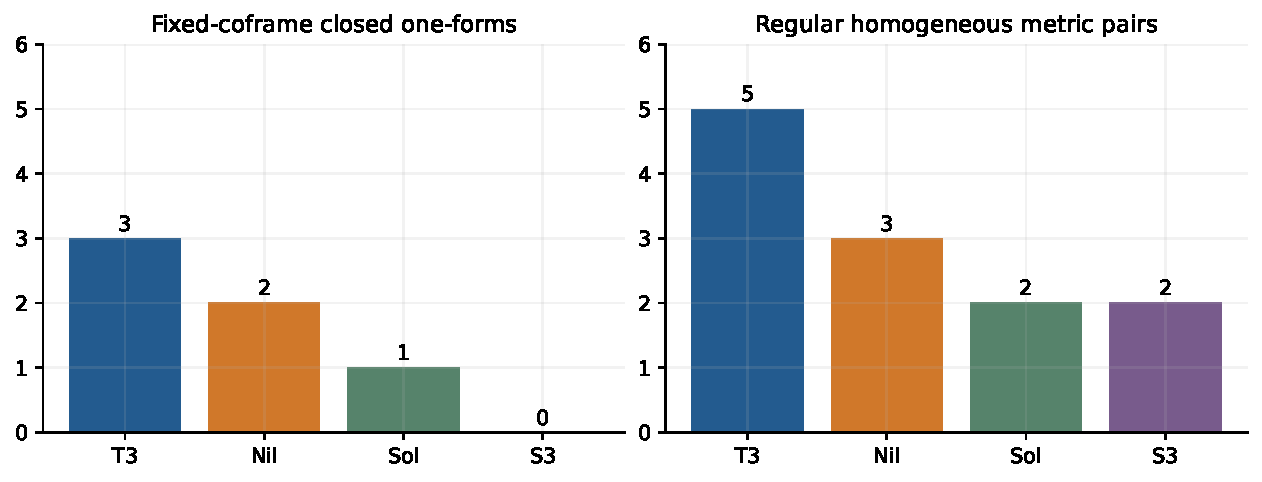
\includegraphics[width=.92\textwidth]{figures/fig01_distinct_counts.pdf}
\caption{Constant closed-one-form dimensions in the specified coframes and homogeneous pair counts on regular constraint strata. The static torus is not on the latter regular stratum.}\label{fig:fig01_distinct_counts}
\end{figure}

\subsection{The singular static torus}

The homogeneous mixed cone and exact family of Paper06, Section 5 and Appendix D, are placed here on the singular stratum of the Hamiltonian constraint $F$ \cite{paper6}. Sections 6--7 add nonzero Fourier components to this setting.

At $n=0$, $\pi=0$, $F$ is quadratic in momenta and $dF=0$. The quadratic action alone retains six metric pairs because its lapse equation vanishes. The second-order coefficient of the original nonlinear Hamiltonian constraint instead imposes the following condition, where $h$ is the first-order mean expansion and $\Sigma$ is tracefree.

\stepcounter{equation}\begin{equation}\tag{T-01}\label{eq:T-01}
K=\varepsilon(hI+\Sigma)+O(\varepsilon^2),\qquad \mathrm{tr}\Sigma=0,\qquad \mathrm{tr}(\Sigma^2)=6h^2.
\end{equation}

This cone is not a vector space. Its pure-scale slice requires $h=0$, while nontrivial simultaneous shape and volume directions exist. Replacing $p_q^2=0$ by $p_q=0$ changes its differential and gauge generator and is not an equivalent regularization.

\stepcounter{equation}\begin{equation}\tag{T-02}\label{eq:T-02}
\begin{aligned}g_{ii}(\tau,\varepsilon)&=q_0^2(1+3\varepsilon h\tau)^{2p_i},\quad p_i=\frac13+\frac{\sigma_i}{3h},\\ \sum_i\sigma_i&=0,\quad\sum_i\sigma_i^2=6h^2,\quad\sum_ip_i=\sum_ip_i^2=1.\end{aligned}
\end{equation}

For $h\ne0$, (T-02) is an exact vacuum solution on $1+3\varepsilon h\tau>0$, and its derivative in $\varepsilon$ realizes the cone direction. A general symmetric $\Sigma$ is recovered by a constant orthogonal matrix representation. If $h=0$, then $\Sigma=0$ and constant metric deformations remain. This explicit homogeneous construction is distinct from the theorem application for spatially dependent waves in Section 7.

The static flat-torus metric family is locally six-dimensional $\mathrm{SPD}(3)$, or five-dimensional at fixed volume, with residual discrete lattice identifications. Its pulled-back symplectic form vanishes because $\pi=0$; this does not make the whole family gauge.


The closed-one-form dimensions of Paper04 and frame comparisons of Paper06 serve as geometric data specifying the homogeneous truncation \cite{paper4,paper6}. Obtaining a reduced metric kernel from those dimensions would additionally require a map to perturbation fields compatible with constraints and gauge quotient. Appendix E collects the preceding geometric results in the present normalization.


\subsection{Linear rank exceptions at Taub points}

At the $S^3$ Taub background (BF-01), the homogeneous momentum rank is two and the full constraint rank is three. Axial $U(1)$ symmetry lowers these from the generic ranks three and four, giving a three-pair linear gauge quotient. This does not replace the two-pair regular-stratum result (H-04). Quadratic KID conditions remain, so the linear quotient is not identified with a smooth nonlinear physical phase space.

The $\ell,m$ tangent directions of the Taub family span one nondegenerate linear pair, while background time displacement is pure gauge. Further KID exceptions occur at low inhomogeneous labels and are counted with their representation multiplicities in Section 6.
